\documentclass[10pt,a4paper]{article}

\usepackage[utf8]{inputenc}		% Configuro la codificación
\input{.command.tex}
% En el siguiente archivo se configuran las variables del trabajo práctico
%% \providecommand es similar a \newcommnad, salvo que el primero ante un 
%% conflicto en la compilación, es ignorado.

% Al comienzo de un TP se debe modificar los argumentos de los comandos

\providecommand{\myTitle}{TRABAJO PRÁCTICO 3} 
\providecommand{\mySubtitle}{Filtro adaptativo}

\providecommand{\mySubject}{Procesamiento de Señales II (86.52)}
\providecommand{\myKeywords}{UBA, Ingeniería, PS2}

\providecommand{\myAuthorSurname}{Manso}
\providecommand{\myTimePeriod}{Año 2018 - 2\textsuperscript{do} Cuatrimestre}

% No es necesario modificar este %%%%%%%%%%%%%%
\providecommand{\myHeaderLogo}{header_fiuba}
%%%%%%%%%%%%%%%%%%%%%%%%%%%%%%%%%%%%%%%%%%%%%%%%

% Si se utilizan listings, definir el lenguaje aquí
\providecommand{\myLanguage}{matlab} 
% Crear los integrantes del TP con el comando \PutMember donde
%%		1) Apellido, Nombre
%%		2) Número de Padrón
%%		3) E-Mail
\providecommand{\MembersOnCover}[0]
{		
		\PutMember{Anastópulos, Matías}{95120}{matias.anas@gmail.com}
		\PutMember{Gasparovic, Emiliano}{96123}{emilianit2000@gmail.com}
		\PutMember{Manso, Juan} {96133} {juanmanso@gmail.com}
}

\providecommand{\myGroupNumber}{02}


\Pagebreaktrue		% Setea si hay un salto de página en la carátula
\Indextrue
\Siunitxtrue			% Si quiero utilizar el paquete, \siunixtrue. Si no \siunixfalse
\Todonotestrue		% Habilita/Deshabilita las To-Do Notes y las funciones \unsure, \change, \info, \improvement y \thiswillnotshow.
\Listingstrue
\Keywordsfalse
\Putgrouptrue		% Habilita/Deshabilita el \myGroup en los headers
\Videofalse
				% Archivo con los comandos globales como Título y autores
%Preambulo para articulo científico de LaTeX

\usepackage[a4paper,left=3cm,right=3cm,bottom=3.5cm,top=3.5cm]{geometry} 	% Configuro la geometría del papel
%\usepackage{microtype}								% Mejora el "spacing" de las palabras
\usepackage[spanish]{babel} 							% Compatibilizo los signos del español
	\addto\captionsspanish{\renewcommand{\tablename}{Tabla}}		%% Redefino nombres preestablecidos por Babel
	\addto\captionsspanish{\renewcommand{\listtablename}{Índice de tablas}}	%% y así en vez de Cuadro dirá Tabla.
\usepackage{amsmath, amsfonts, amssymb}						% Entornos matemáticos, fuentes y símbolos
\usepackage{graphicx}								% Necesario para insertar figuras
\usepackage{fancyhdr}								% Para manipular headers y footers
\usepackage[usenames,dvipsnames]{color}						% \color{color deseado} {lo que querés que tenga color}
\usepackage{subcaption}								% Permite captions del tipo 1a, 1b
\usepackage{multirow}								% Para tablas
\usepackage{float}

% Para video
\ifVideo
	\usepackage{media9}
	\addmediapath{./../reportes/}
\fi

%\usepackage{times}
%\usepackage{mathtools}
%\usepackage{upgreek} % letras griegas sin cursiva
%\usepackage{cancel}
\usepackage{rotating}
\usepackage{tikz}
\usepackage{pgfplots}
%	\pgfplotsset{compat=1.12}
	\usetikzlibrary{plotmarks}% matlab2tikz
\usepackage{grffile}% matlab2tikz 
	\usetikzlibrary{calc,patterns,decorations.pathmorphing,decorations.markings}

\ifListings
	\usepackage{listings}

	\providecommand{\lstinputpath}[1]{\lstset{inputpath=#1}}

%	\input{.lst_default.tex}
	\input{.lst_matlab.tex}
%	\input{.lst_c.tex}
%	\input{.lst_c++.tex}
	
% 	\input{.lst_pseudocode.tex}


\fi

\ifSiunitx
\usepackage{siunitx}											% Unidades: \SI {cantidad} {\unidad} (necesita texlive-science)
	\sisetup{load-configurations = abbreviations}							% Habilita poner \cm en vez de \centi\metre
	\sisetup{output-decimal-marker = {,}}									% Cambia los puntos decimales por comas
	\sisetup{per-mode = fraction}											% Pone las unidades como fracción
	\sisetup{quotient-mode = fraction}										
\fi


\ifTodonotes
\usepackage{xargs}
\usepackage[colorinlistoftodos,prependcaption,textsize=tiny]{todonotes}


	\newcommandx{\Juan}[2][1=]{\todo[linecolor=blue,backgroundcolor=blue!25,bordercolor=blue,#1]{#2}}
	\newcommandx{\Mati}[2][1=]{\todo[linecolor=green,backgroundcolor=green!25,bordercolor=green,#1]{#2}} % OliveGreen
	\newcommandx{\Emi}[2][1=]{\todo[linecolor=Plum,backgroundcolor=Plum!25,bordercolor=Plum,#1]{#2}}
	\newcommandx{\unsure}[2][1=]{\todo[linecolor=red,backgroundcolor=red!25,bordercolor=red,#1]{#2}}
	\newcommandx{\thiswillnotshow}[2][1=]{\todo[disable,#1]{#2}}
\fi


\usepackage{booktabs}														% Permite hacer tablas sin separadores en el medio
\usepackage{placeins}														
		\let\Oldsection\section												%% Permite que los flotantes (como figuras) no aparescan
	\renewcommand{\section}{\FloatBarrier\Oldsection}						%% antes o después de su sección correspondiente.
		\let\Oldsubsection\subsection
	\renewcommand{\subsection}{\FloatBarrier\Oldsubsection}		
		\let\Oldsubsubsection\subsubsection
	\renewcommand{\subsubsection}{\FloatBarrier\Oldsubsubsection}
\usepackage{hyperref}														% Debe ser agregado al final del preambulo

\hypersetup
{    bookmarks=true,         % show bookmarks bar?
     unicode=false,          % non-Latin characters in Acrobat’s bookmarks
     pdftoolbar=true,        % show Acrobat’s toolbar?
     pdfmenubar=true,        % show Acrobat’s menu?
     pdffitwindow=false,     % window fit to page when opened
     pdftitle={\myTitle},    		 % title
     pdfauthor={\myAuthorSurname},   % author
	 pdfcreator={\myAuthorSurname},	 % creator = author
     pdfsubject={\mySubject},		 % subject of the document
     pdfkeywords={\myKeywords},
     colorlinks=true,        % false: boxed links; true: colored links
     linkcolor=black,        % color of internal links (change box color with linkbordercolor)
     citecolor=black,        % color of links to bibliography
     filecolor=magenta,      % color of file links
     urlcolor=cyan           % color of external links
}

%Configuro la pagina con los encabezaos y pies de paginas
\pagestyle{fancy}										% Para agregar encabezados y pie de paginas	
\lhead{\mySubject}										% Encabezado izquierdo
\rhead{\includegraphics[scale=0.15]{\myHeaderLogo}} 	% Encabezado derecho (logo de la FIUBA)	
\ifPutgroup
\chead{\texttt{Grupo Nº\myGroupNumber} }%\\ \textit{\footnotesize{\myTimePeriod}}}
\fi				

%% Este archivo contiene las funciones auxiliares para escribir en LaTeX
%% Dichas funciones resuelven la sintaxis de generar figuras, por ejemplo,
%% dejando el código más compacto y facilitando la corrección del mismo.



% Comando para graficar eps. 1er arg, escala. 2do, ruta. 3ro, caption. 4to, label.
\providecommand{\HgraficarEPS}[4]{
			\begin{figure}[h!]
				\centering
					\scalebox{#1}{\input{#2}}
					\caption{#3}
					\label{#4}
			\end{figure}

}

\providecommand{\HgraficarPNG}[4]{
			\begin{figure}[h!]
				\centering
					\includegraphics[scale=#1]{#2}
					\caption{#3}
					\label{#4}
			\end{figure}

}


% Comando para graficar eps en el lugar previsto.
\providecommand{\graficarEPS}[4]{
			\begin{figure}[h]
				\centering
					\scalebox{#1}{\input{#2}}
					\caption{#3}
					\label{#4}
			\end{figure}

}

\providecommand{\graficarPNG}[4]{
			\begin{figure}[h]
				\centering
					\includegraphics[scale=#1]{#2}
					\caption{#3}
					\label{#4}
			\end{figure}

}

\providecommand{\graficarPDF}[3]{
			\begin{figure}[h!]
				\centering
		\includegraphics[width=1.0\textwidth,keepaspectratio]{#1}
					\caption{#2}
					\label{#3}
			\end{figure}

}


\providecommand{\graficarPDFwide}[3]{
			\begin{figure}[h!]
				\centering
		\includegraphics[scale=0.5,trim={6,5cm 0 0 0}]{#1}
					\caption{#2}
					\label{#3}
			\end{figure}

}

\providecommand{\graficarPDFa}[4]{
			\begin{figure}[h!]
				\centering
				\includegraphics[scale=0.5,trim={#1}]{#2}
					\caption{#3}
					\label{#4}
			\end{figure}

}



\providecommand{\underuparrow}[2]{\underset{\underset{#2} \uparrow} #1 }

\providecommand{\cltext}[2]{\color{#1}{\huge{#2}}}

\providecommand{\cstext}[2]{\color{#1}{\large{#2}}}

\providecommand{\vect}[1]{\boldsymbol{#1}}
\providecommand{\dvect}[1]{\dot{\boldsymbol{#1}}}
\providecommand{\dd}{\mathrm{d}}
		% Se proveen un conjunto de funciones extras

% Defino el path de los includegraphics
\graphicspath{{./Figuras/}}		% Directorio que contiene los graficos

% Defino el path para los input de .tex y de .eps
\makeatletter
\def\input@path{{./Figuras/}{./Secciones/}{./Cover_page/}}
\makeatother

% Defino el path del listings
\ifListings
%% Cambiar el nombre de la carpeta si se utilizan Listings
	\lstinputpath{{../Octave/}}
\fi

\definecolor{myred}{rgb}{0.5,0,0}
\definecolor{mygreen}{rgb}{0,0.5,0}

\renewcommand{\thesubsection}{\thesection.\alph{subsection}}

\begin{document}
		% Carátula (formal o simple,_formal o _simple respectivamente) con Resumen
		% incluido e Índice (si es necesario configurar en config.tex) del informe
		\begin{titlepage}
	
		\thispagestyle{empty}

		\begin{center}
			
\includegraphics[scale=0.3]{fiuba}\\
			\large{\textsc{Universidad de Buenos Aires}}\\
			\large{\textsc{Facultad De Ingeniería}}\\
			\small{\myTimePeriod}
		\end{center}

		\vfill

		\begin{center}
			\Large{\underline{\textsc{\mySubject}}}
		\end{center}

		\vfill

		\begin{tabbing}
			\hspace{2cm}\=\+\myTitle\\
				TEMA: \mySubtitle\\
				FECHA: \today\\
			\\
				\MembersHeader
				\MembersOnCover	
		\end{tabbing}

		\begin{abstract}
			% Ejemplo de Resumen
%% MANTENER EL NOMBRE %%
	El presente trabajo tiene como objetivo utilizar el filtro de Kalman para estimación de trayectorias y analizar sus modificaciones ante diversas condiciones.

		\end{abstract}

	\ifKeywords
		\begin{center}
			\emph{Palabras Clave: \myKeywords}
		\end{center}
	\fi	

		\vfill
	
\end{titlepage}

\ifPagebreak
	\thispagestyle{empty}
	\ifIndex
		\tableofcontents
%		\listoffigures
%		\listoftables
	\fi

	\pagebreak
\fi


	\setcounter{page}{1}

\begin{center}{\Large{\textbf{Enunciado}}}\end{center}
%	Filtro adaptativo
\emph{Steepest Desend}	
	\begin{equation*}
		\hat{w}(n+1) = \hat{w}(n) + \mu\,p
	\end{equation*}
	donde $\mu$ regula velocidad (paso) y $p = -\nabla\, J(\hat{w}(n)) = 2p - 2R\,\omega(n)$ con $\mu > 0$ y $M = I$.

LMS (gradiente estocástico)
	\begin{align*}
		\hat{w}(n+1) &= \hat{w}(n) - \mu\, 2(-\hat{p} + \hat{R}\,\hat{w}(n))\\
		\hat{R} &= u(n) \, u^{H}(n)\\
		\hat{p} &= u(n) \, d^{*}(n)
	\end{align*}

Características de los filtros adaptativos:
	\begin{enumerate}
		\item Velocidad de convergencia
		\item Desajuste (diferencia entre J y J de Wiener) [\emph{Mismatch}]
		\item Rastreo [\emph{Tracking}] (si mi sistema tiene características que cambian con el tiempo, que pueda seguirlas)
		\item Robustez (para pequeños errores que el resultado me de con pequeños errores
	\end{enumerate}

	En base a estas características se elige el filtro adaptativo.

	\begin{equation*}
		\begin{cases}
			i(n) = A_0 \sen (\omega_0 \, n + \theta)\\
			u(n) = A_1 \sen (\omega_0 \, n) & \text{con $\theta=0$}
		\end{cases}
	\end{equation*}

\subsection{Ejercicio 1}
	Analice desde el punto de vista de la estimación lineal óptima el problema genérico de cancelar una señal de referecia correlacionada con la misma. ¿Cuál es la señal de error? ¿Qué otras hipótesis pueden ser necesarias? (Parecido a uno del cuatri pasado de cancelación de ruido)
	\begin{equation*}
		\begin{cases}
			d(n) = i(n)\\
			d(n) = s(n) + i(n)
		\end{cases}
	\end{equation*}

	\underline{\Large{Respuesta}}\\
	\graficarPNG{0.4}{Wiener2}{Diagrama en bloques del problema.}{fig:bloques_wiener}
	
	Si $d[n]=i[n]$ 
	

\subsection{Ejercicio 2}
	Implemente un LMS para cancelar i(n) y escuchar el audio lo mejor posible.\\
	a) Reescribir el algoritmo en función del error $e(n)$
		\begin{equation*}
			\underline{\hat{w}}(n+1) = \underline{\hat{w}}(n) + \mu^{'} \underline{u}(n)\, e^{*}(n)
		\end{equation*}

	b) Varie $\mu$ (a veces tarda más a veces menos en converger y a veces no llega a nada)
	
	c) Varie el rango del filtro (L)
	
	d) A mitad de la simulación tiene que cambiar de forma abrupta cada uno de los parámetros ($A_0$ $\omega_0$ y $\theta$). Grafique el error absoluto, los coeficientes (deberíamos ver que convergen) y la canción con la canción estimada.


	\underline{\Large{Respuesta}}\\

	


	El objetivo del trabajo será la implementación de un algoritmo de identificación de un sistema fisico determinado. El sistema a identificar puede verse en la figura \ref{fig:auto}, se trata de un sistema de amortiguación de un automovil.

\vspace*{\fill}
\begin{figure}[H]
\centering
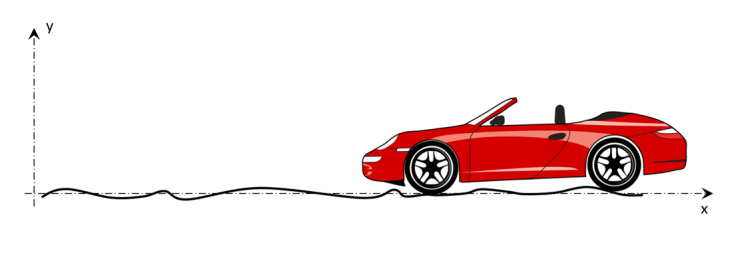
\includegraphics[scale=0.7]{auto.png}
\caption{Sistema Fisico.}
\label{fig:auto} 
\end{figure}
\vspace*{\fill}

El modelo a utilizar para identificar el sistema es el que observamos en la figura \ref{fig:mbk}. Se trata de un sistema de masa, amortiguador y resorte, donde la entrada $x_{1}$ es el nivel del suelo, y la salida $x_{2}$ es la altura en la que se encuentra el chasis del automovil. La idea es, mediante un filtro adaptativo, poder estimar las constantes $m$, $b$ y $k$ del sistema.

\vspace*{\fill}
\begin{figure}[H]
\centering
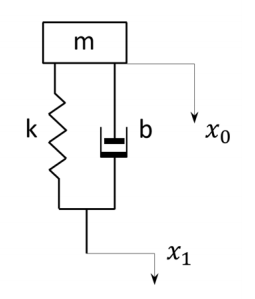
\includegraphics[scale=0.6]{mbk.png}
\caption{Modelo.}
\label{fig:mbk} 
\end{figure}
\vspace*{\fill}

	
	\section{Modelado y discretización}\label{sec:ej1}
	La ecuación del sistema de masa, resorte y amortiguador es la siguiente:

\begin{equation*}
	m \ddot{x}_{0}(t) + k (x_{0}(t) - x_{1}(t)) + b (\dot{x}_{0}(t) - \dot{x}_{1}(t)) = 0
\end{equation*}

Para poder discretizar el mismo se utilizaron las siguientes aproximaciones:

\begin{equation*}
	\dot{x}_{0} \approx \frac{x_{0}(n + 1) - x_{0}(n)}{\Delta T}
\end{equation*}

\begin{equation*}
	\ddot{x}_{0} \approx \frac{x_{0}(n + 1) - 2 x_{0}(n) + x_{0}(n - 1)}{\Delta T^2}
\end{equation*}

\begin{equation*}
	\dot{x}_{1} \approx \frac{x_{1}(n + 1) - x_{1}(n)}{\Delta T}
\end{equation*}
donde $\Delta T$ es el período de muestreo. Con todas las aproximaciones anteriores, y la ecuación del sistema en tiempo continuo, se llega a la siguiente ecuación en diferencias para el tiempo discreto.

\begin{equation*}
	x_{0}(n) = \frac{b \;\Delta T}{m + b \;\Delta T} x_{1}(n) + \frac{k \;\Delta T^2 - b \;\Delta T}{m + b \;\Delta T} x_{1}(n - 1) - \frac{k \;\Delta T^2 - 2 m - b \;\Delta T}{m + b \;\Delta T} x_{0}(n - 1) - \frac{m}{m + b \;\Delta T} x_{0}(n - 2)
\end{equation*}


		
	\section{Filtro adaptativo}\label{sec:ej2}
	
	Se presenta el esquema del filtro propuesto en la Figura \ref{fig:filtro_adaptativo}. 
	Ambos sistemas (el desconocido y el filtro adaptativo) se excitan con una señal de referencia $u(n)$ de ruido blanco gaussiano.
	Luego se computa la diferencia entre ambas salidas y se utiliza esta señal de error para el ajuste de los parámetros del filtro mediante algún algoritmo adaptativo.
	Cuando el filtro aprenda a comportarse igual que el sistema a identificar, el error será bajo, y los coeficientes del filtro podrán utilizarse como estimadores de los parámetros del sistema a identificar.

\vspace*{\fill}
\begin{figure}[H]
\centering
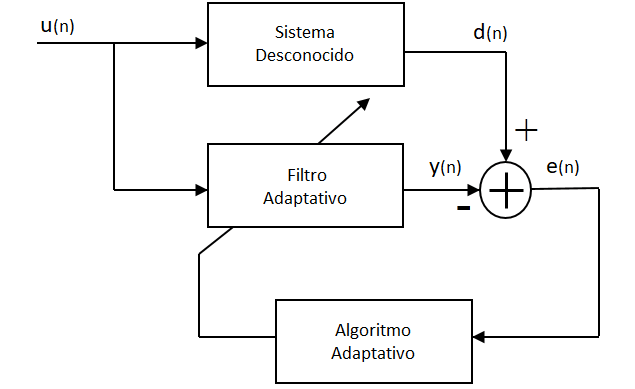
\includegraphics[scale=0.5]{filtro_adaptativo.png}
\caption{Filtro Adatptativo.}
\label{fig:filtro_adaptativo} 
\end{figure}
\vspace*{\fill}

Sin embargo ésto tiene un problema. La salida del filtro adaptativo se computa de la siguiente manera:
\begin{equation*}
	y(n) = w^T U(n)
\end{equation*}
donde $U(n) = [u(n) \> u(n - 1) \> ... \> u(n - M + 1)]^T$, $M$ es el orden del filtro y $w$ son los coeficientes del mismo.

	Ésto significa que el filtro adaptativo propuesto sólo sirve para estimar la respuesta en frecuencia de sistemas FIR y el sistema bajo análisis tiene la forma de un filtro IIR en tiempo discreto:

\begin{equation*}
		x_{0}(n) = b_{0} \> x_{1}(n) + b_{1} \> x_{1}(n - 1) + a_{0} \> x_{0}(n - 1) + a_{1} \> x_{0}(n - 2)
\end{equation*}

Una posible solución a esto es, en lugar de sólo introducir ruido blanco a la entrada, combinar el ruido blanco con algunos valores pasados de la salida:

\begin{equation*}
	U(n) = [x_{1}(n) \> x_{1}(n - 1) \> x_{0}(n - 1) \> x_{0}(n - 2)]^T
\end{equation*}
donde ahora se excita al sistema con $x_{1}$ ruido blanco gaussiano. Así los coeficientes $w$ ajustados del filtro podrán utilizarse como estimadores:

\begin{equation*}
	[w_{0} \> w_{1} \> w_{2} \> w_{3}]^T  = [\hat{b}_{0} \> \hat{b}_{1} \> \hat{a}_{0} \> \hat{a}_{1}]^T
\end{equation*}

Ahora bien, como estos coeficientes son función de las constantes $m$, $b$ y $k$, pueden estimarse las mismas. El único componente que falta es la elección del algoritmo adaptativo. Se propone en principio utilizar el algoritmo LMS, que obtiene los parámetros $w$ de la siguiente manera:

\begin{equation*}
	w(n) = w(n - 1) + \mu \> U(n) \> [d(n) - U(n)^* w(n - 1)]
\end{equation*}

donde $\mu$ es una constante de aprendizaje.


	\section{Implementación del filtro adaptativo}\label{sec:ej3}
			
	A continuación se presenta el \emph{script} con la implementación del algorítmo. 
	\lstinputlisting[linerange=Implementacion-fin]{ej_3.m}

	En la Figura \ref{fig:ej3} se expone la convergencia de los coeficientes en función de la cantidad de muestras (tiempo). Se puede ver que para más de 300 muestras, la estimación es correcta. Sin embargo al presentarse ruido en la medición de la salida, la estimación fluctúa alrededor del valor correcto. 
	\Juan{No estoy seguro que esté taaan bien}
	Si la incertidumbre de la medición es muy grande, la estimación tardará más en converger y oscilará en un rango mayor entorno al verdadero.

	\begin{figure}[h!]
		\centering
		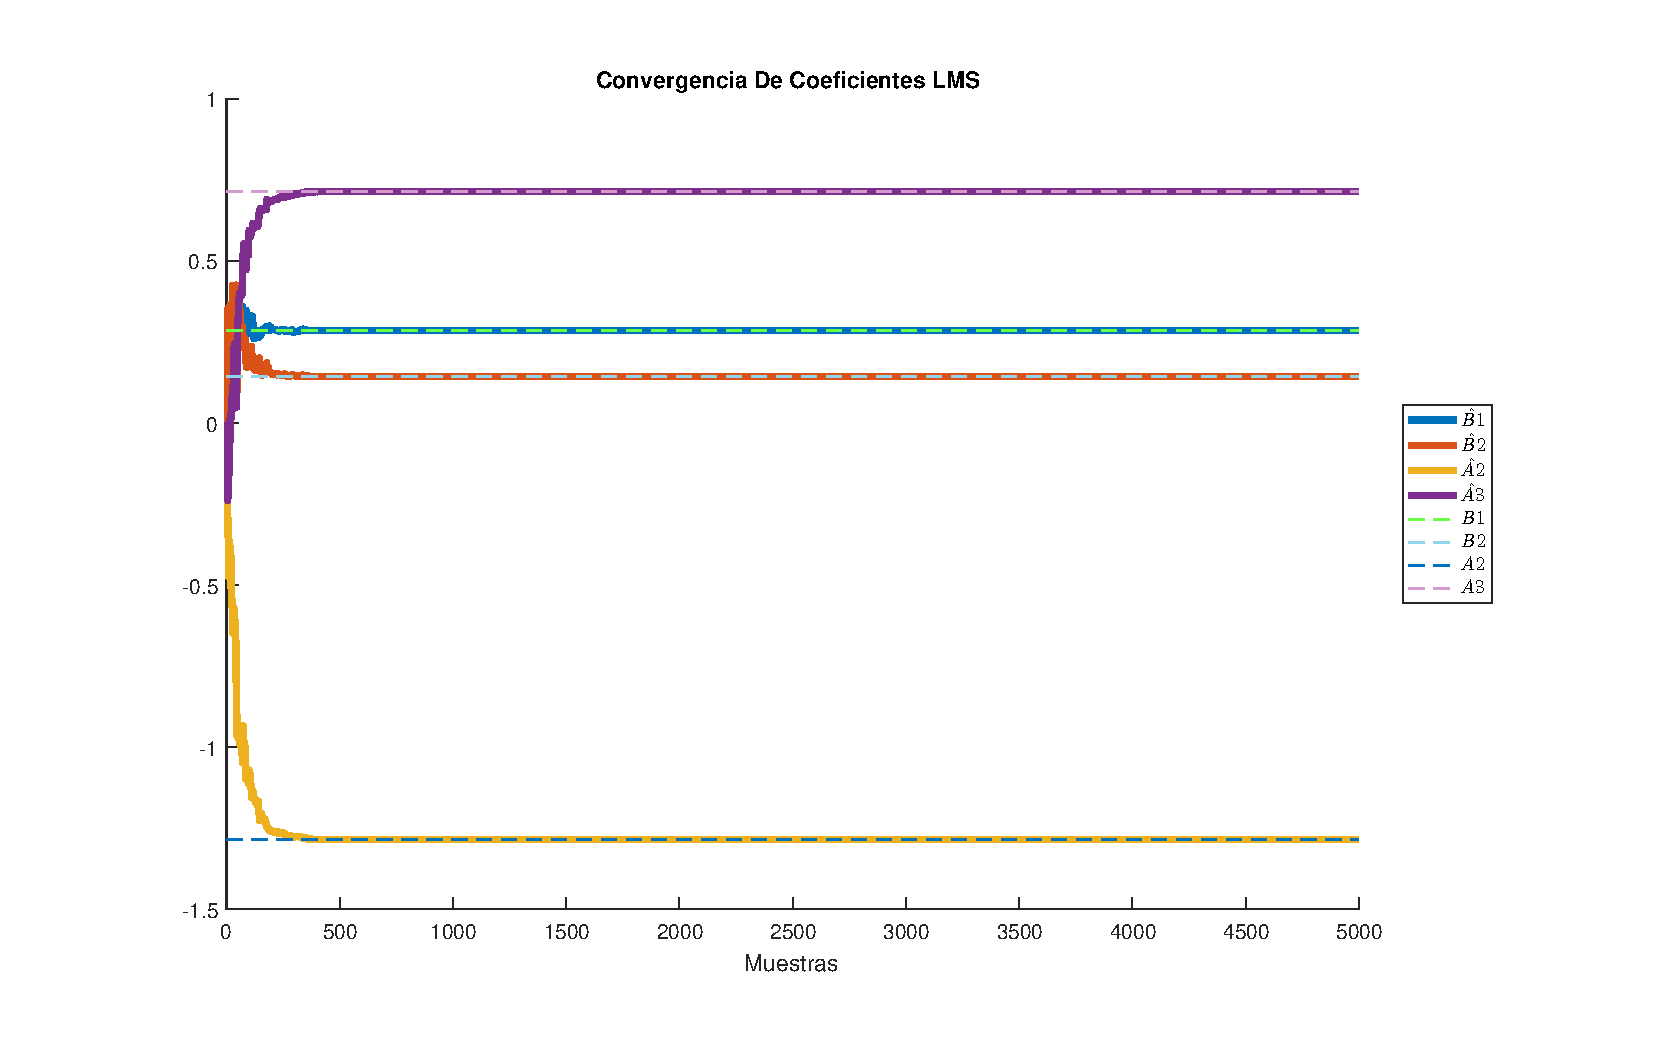
\includegraphics[width=1.0\textwidth, trim = 0cm 0cm 0cm 0cm]{graf_ej3.pdf}
		\caption{Convergencia de los coeficientes a partir de la estimación LMS.}
		\label{fig:ej3}
	\end{figure}

	\lstinputlisting[linerange=Resultados- ]{ej_3.m}
	Los resultados de la simulación a través de la función \texttt{solve()} se exponen en la siguiente tabla: 

		\begin{table}[h!]
			\centering
			\begin{tabular}{ccc}
				\toprule
				$m$ (fija)	& $k$	& $b$\\
				\midrule
				5&\num{2.9849}&\num{1.9972}\\
				\bottomrule
			\end{tabular}
			\caption{Resultados de la estimación de los parámetros.}
			\label{tab:res_ej3}
		\end{table}

		\Juan{No sé qué poner ahí}
	Se puede ver que los errores son del orden del 1\% siendo este valor muy bajo.





	\pagebreak
	\section{Comportamiento ante corte del resorte}\label{sec:ej4}
		

\graficarPDF{graf_ej4}{graf\_ej4}{fig:ej4}
\graficarPDF{graf_ej4_covinn}{Innovaciones ej4}{fig:4covinn}
\graficarPDF{graf_ej4_pos}{Posición ej4}{fig:4pos}
\graficarPDF{graf_ej4_theta}{Theta ej4}{fig:4theta}
\graficarPDF{graf_ej4_vel}{Velocidad ej4}{fig:4vel}


	\pagebreak
	\section{Filtro \emph{NLMS}}\label{sec:ej5}
		
% Acá entran los puntos 5 y 6

	
	



	\begin{figure}[h!]
		\centering
		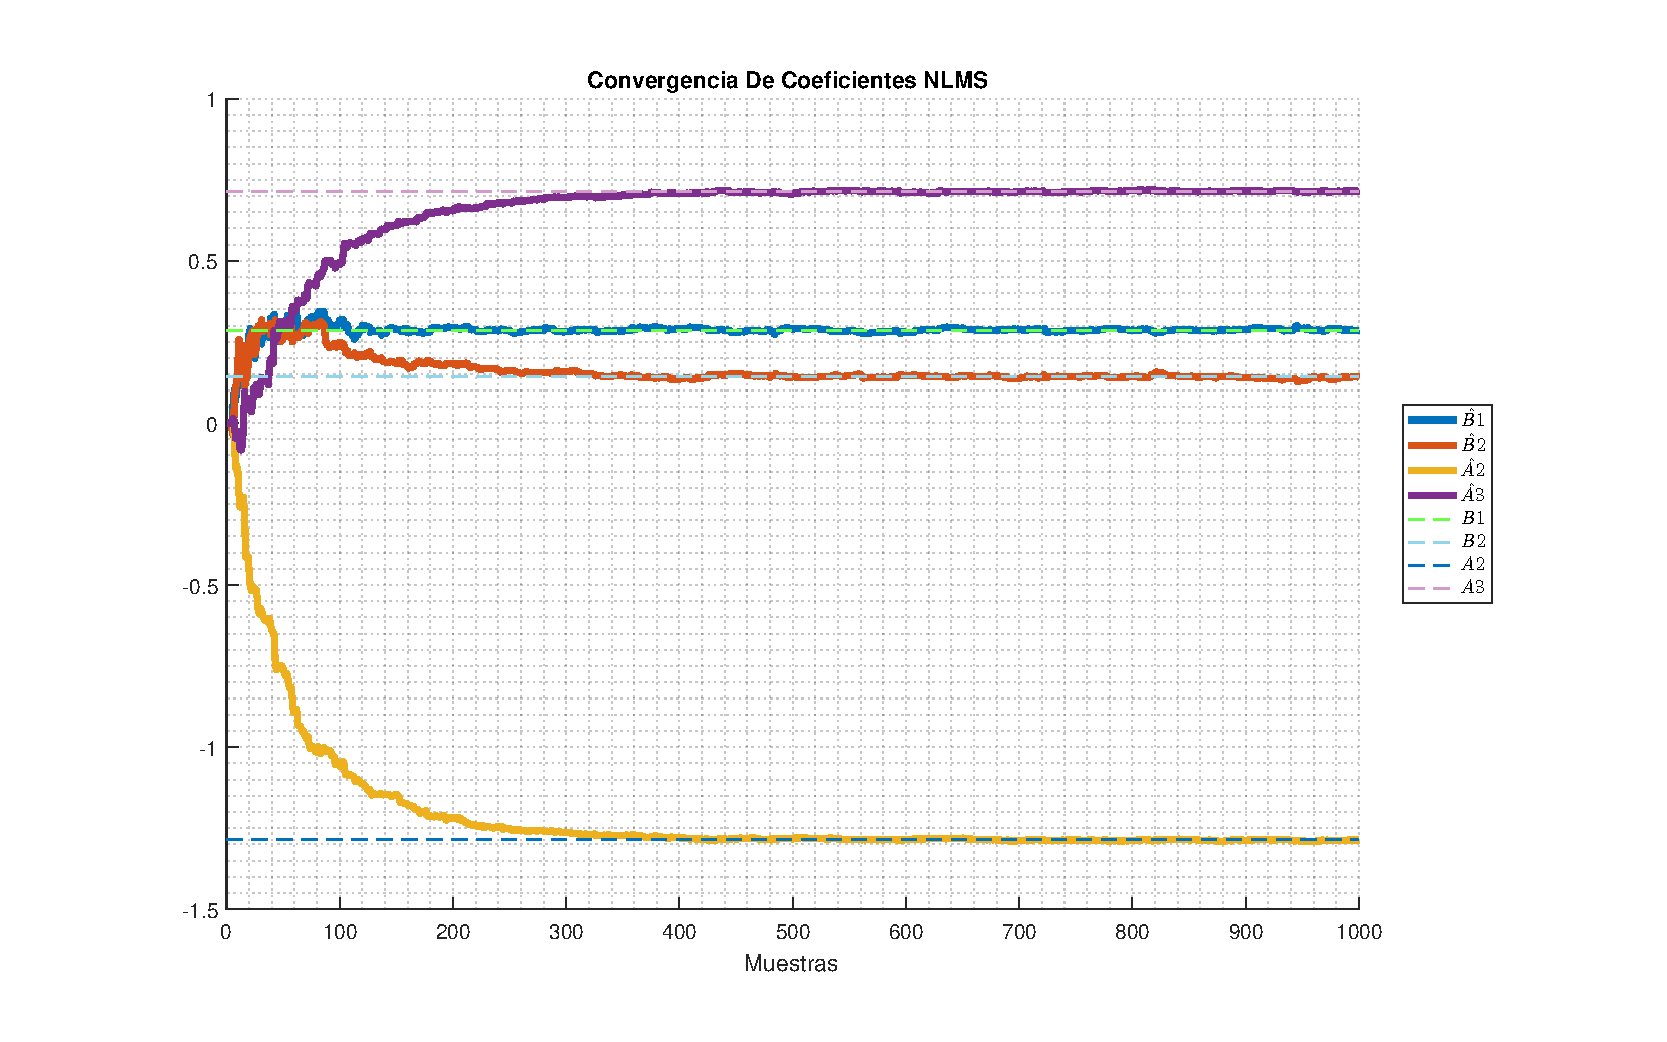
\includegraphics[width=1.0\textwidth]{graf_ej5.pdf}
		\caption{Convergencia de los parámetros a partir de la estimación LMS.}
		\label{fig:ej3}
	\end{figure}


	\begin{figure}[h!]
		\centering
		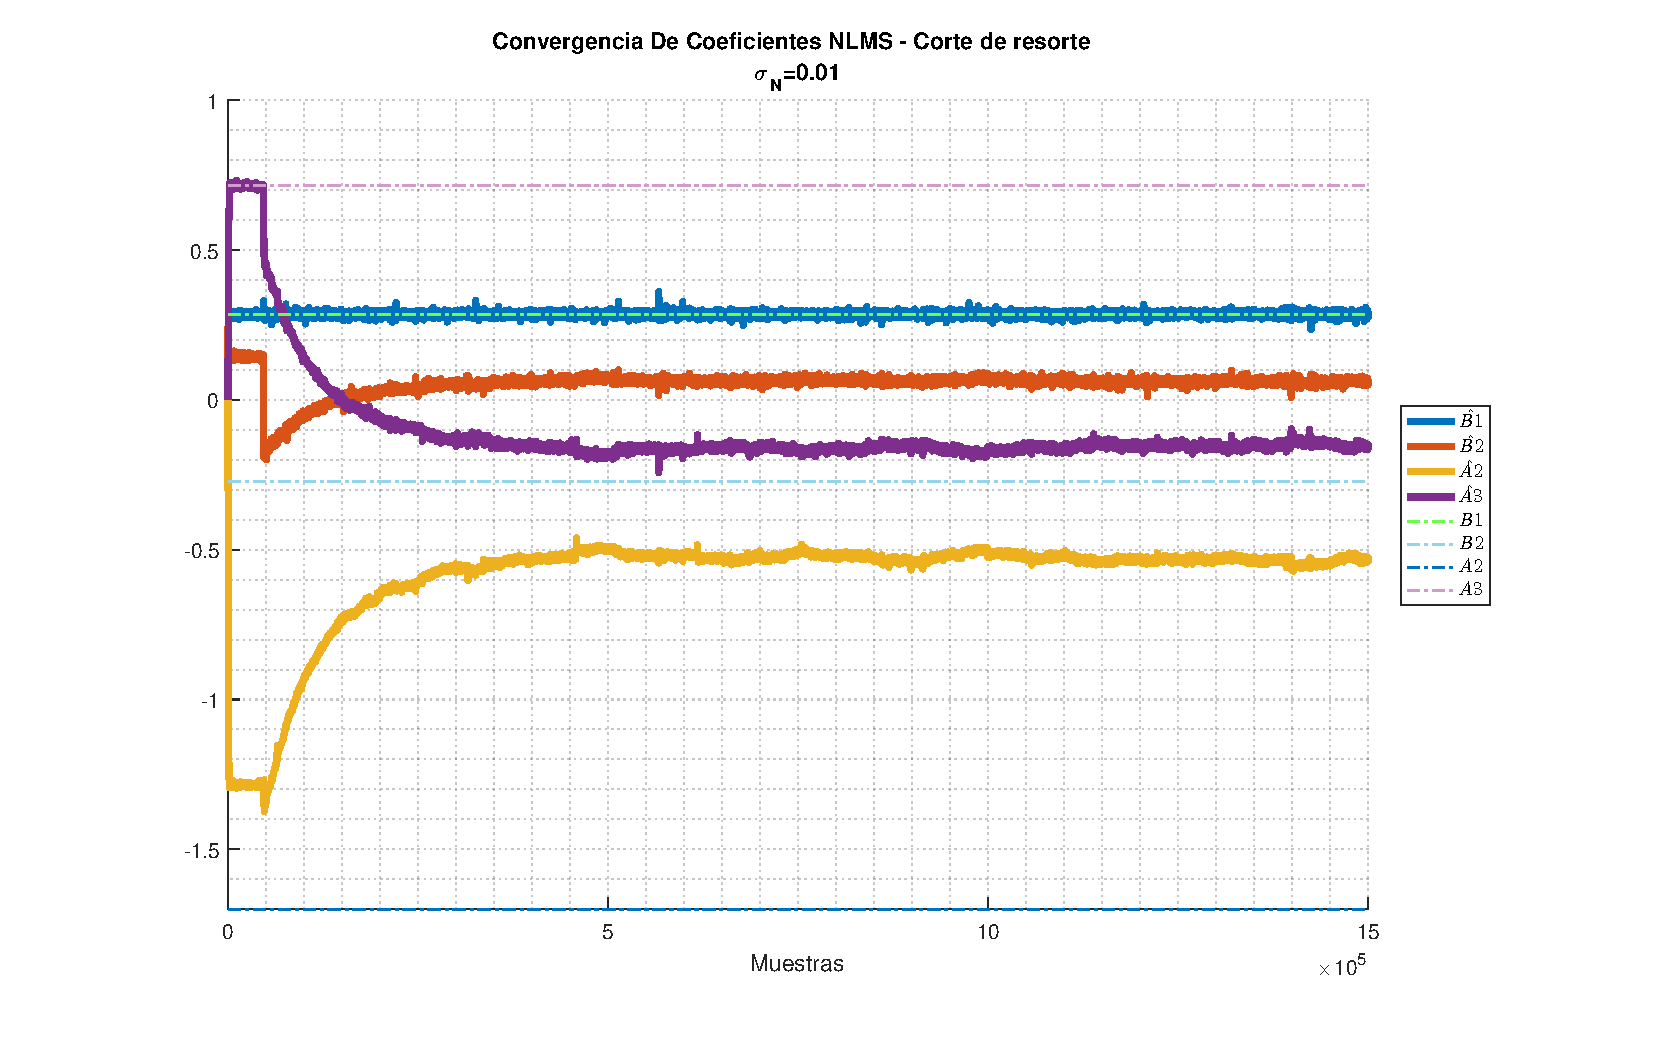
\includegraphics[width=1.0\textwidth]{graf_ej5_k0.pdf}
		\caption{Convergencia de los parámetros a partir de la estimación LMS.}
		\label{fig:ej3}
	\end{figure}




	\section{Conclusiones}\label{sec:conclusiones}
		\paragraph{}
Se observa en el presente trabajo la utilidad de los filtros adaptativos como sistemas de identificación. Mediante un algoritmo iterativo, se puede obtener un filtro cuyos coeficientes se asemejan a los del modelo del sistema físico real. Se observa como, con el paso del tiempo, el filtro converge a los valores correctos, mejorando el error en cada iteración.
\paragraph{}
Sin embargo, también se observa como el ruido de medición puede afectar severamente la convergencia del algoritmo, y por lo tanto, los resultados finales. Si el mismo es demasiado alto, los coeficientes no convergerán a los valores correctos.
\paragraph{}
Por otro lado, se observa la capacidad del algoritmo de adaptarse a la situación presente. Como por ejemplo, cuando se corta el resorte, los coeficientes modifican su tendencia, dirigiéndose a los nuevos valores correctos. Se observó también, que la velocidad de convergencia del algoritmo puede ser afectada severamente cuando el resorte se corta.



	% \appendix
\end{document}
